% Native English captures; see docs/provenance/english-edition-assets.json for source and crop metadata.
\begin{figure}[H]
\centering
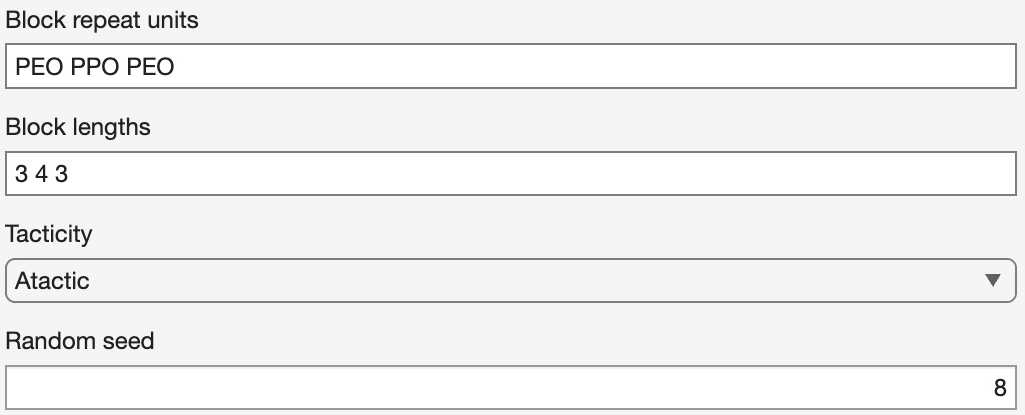
\includegraphics[width=\linewidth]{publication-assets/crop-3d7aab6f859860340b2f.png}
\par\vspace{3mm}
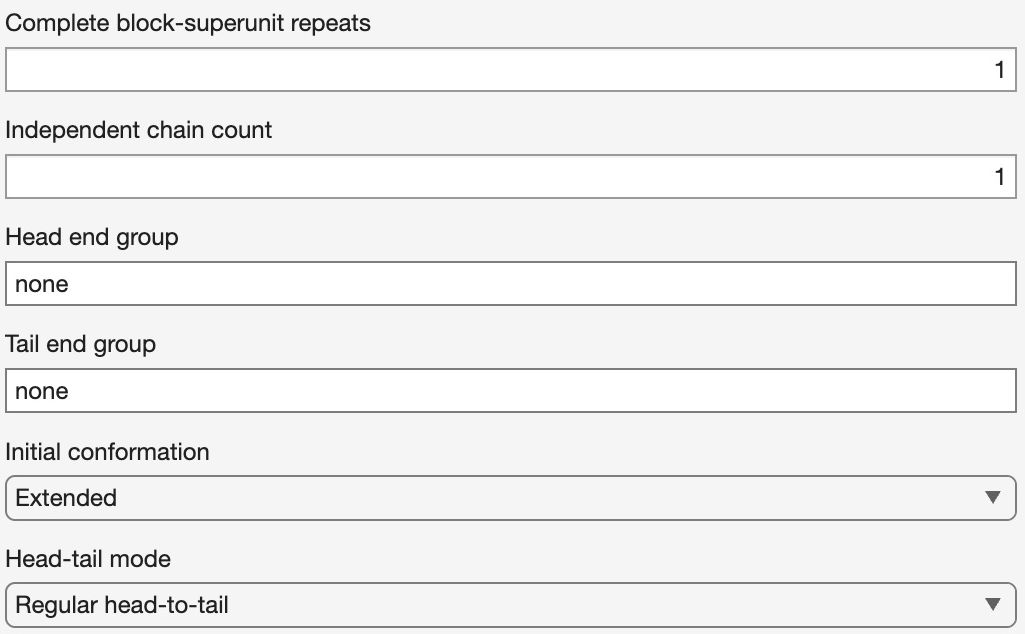
\includegraphics[width=\linewidth]{publication-assets/crop-14436d05d0623e7cdc6f.png}
\caption{Parameters for a PEO--PPO--PEO block chain. Above: \literalinput{PEO PPO PEO}, \literalinput{3 4 3}, and seed 8. Below: one repeat, one chain, both end groups \file{none}, an extended starting conformation, and regular head-to-tail connections.}
\label{fig:polymer-block-parameters}
\end{figure}

\begin{figure}[H]
\centering
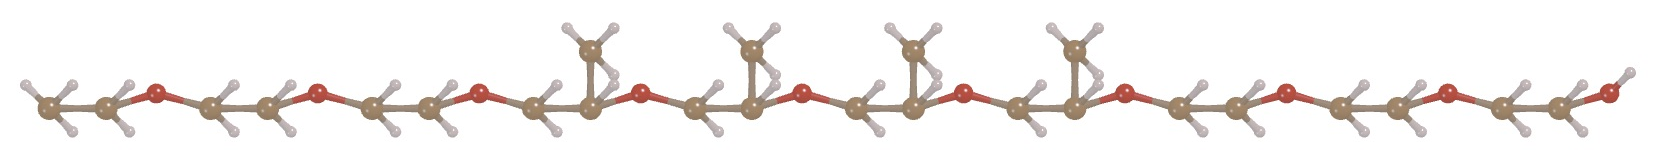
\includegraphics[width=\linewidth]{publication-assets/crop-7684a8a790954b6a1954.png}
\par\vspace{3mm}
\begin{minipage}[t]{40mm}
\vspace{0pt}
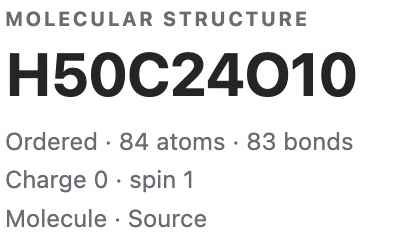
\includegraphics[width=\linewidth]{publication-assets/crop-c77f26280735587ce6a4.png}
\end{minipage}\hfill
\begin{minipage}[t]{80mm}
\vspace{0pt}
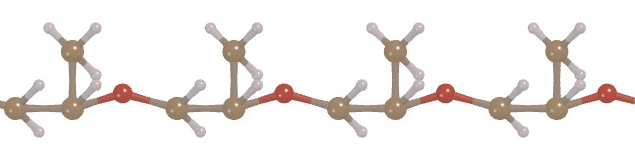
\includegraphics[width=\linewidth]{publication-assets/crop-71a6b6056b817444ef97.png}
\end{minipage}
\caption{The resulting initial block chain. Above: the complete chain. Below left: $\mathrm{C_{24}H_{50}O_{10}}$, 84 atoms, and 83 connections. Below right: the four methyl branches in the central PPO block.}
\label{fig:polymer-block-model}
\end{figure}
